\chapter{基于规则与案例的医疗方案推荐方法}

本章主要介绍基于规则的医疗方案推荐方法以及基于案例的医疗方案推荐方法。首先,考虑到对于算法的研究都依赖于数据,本章先介绍所有研究的数据来源与背景,详细讨论的数据的格式。随后本问介绍了如何精简数据中的信息,如何选取研究所依赖的属性。最后再来详细介绍基于规则与案例的几种医疗方案推荐算法。值得注意的是,本文涉及的医疗方案主要针对乳腺癌这一种疾病,但所使用的模型与思想具有普适性。

\section{病例数据}
\label{sec_3_1}
\subsection{病例数据简介}
为了对本文的模型与思想加以验证,一个完善的临床病例数据库十分必要。本文所使用的所有研究数据均来源于上海交通大学附属瑞金医院乳腺中心。该中心成立于2009年2月,科室依托于上海交通大学医学院附属瑞金医院,与肿瘤放化疗科,病理科,放射诊断科,超声诊断科,核医学科和整形外科等多学科群综合整合成为乳腺疾病诊治中心,是致力于乳腺疾病预防,诊断与治疗的医疗,教学和科研机构。中心牵头,联合国内多家医院共同维护了一个内容丰富详细的乳腺癌临床病例数据库。该数据库详细的记录了所有参与多学科讨论的病人的以下几类信息:
\begin{itemize}

\item 基本信息,家庭信息,遗传信息,既往病史。
\item 各种理化指标。包括血检,生理实验结果等。
\item 参与的各种治疗类型,包括化疗,放疗,内分泌治疗,靶向治疗等。
\item 治疗方案。一般治疗方案为已经成熟的一套治疗计划,包括疗程数,各疗程时长,以及每个疗程用药量等信息。针对每个病人的某种治疗类型,医生从既有的几种治疗方案中选择一个。
\item 疗效信息,包括是否治愈,治愈后是否复发,复发后是否死亡等。

\end{itemize}

从2016年9月至近,已经有陆续8000个左右病例被加入数据库,本文的研究正是证实基于这些数据展开的。

\subsection{病例数据库结构}
在该临床病例数据库中,最核心的表是患者表,这张表上记录着所有入库的病人的基本信息。还有许多从病人表衍生出的表共同丰富了整个临床数据库的信息。所有这些表有属于病人表。这些表包括患者既往史表、组织活检病理学表、手术病理表与病灶表、影像学检查表、患者临床指标表、随访信息表、新辅助治疗方案表。表之间的的结构图如图\ref{fig:ch3-1}所示。患者表与各个表之间的从属关系如表\ref{tab:3-1}所示。



\begin{figure}[!htp]
  \centering
  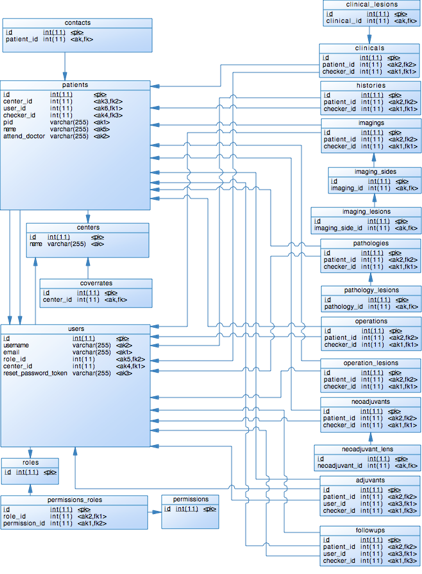
\includegraphics{figure/chap3-1_database_schema.png}
  \bicaption[病例数据库结构]
    {病例数据库结构}
    {the basic structure of the physical data}
  \label{fig:ch3-1}
\end{figure}



% \begin{figure}[!htp]
%   \centering
%   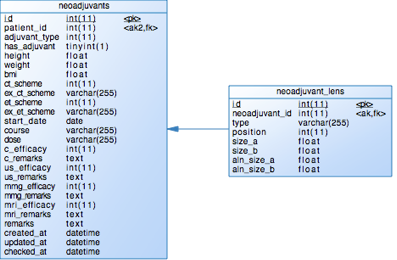
\includegraphics{figure/chap3-7_neoadjuvants.png}
%   \bicaption[新辅助治疗方案]
%     {新辅助治疗方案}
%     {schema of neoadjuvants}
%   \label{fig:ch3-7}
% \end{figure}

\begin{figure}[!htp]
  \centering
  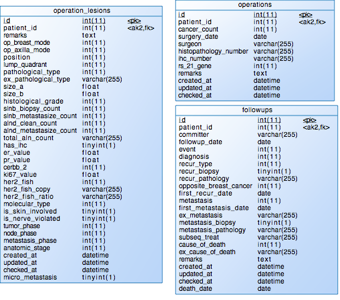
\includegraphics{figure/chap3-6_operations.png}
  \bicaption[手术病理及手术病灶]
    {手术病理及手术病灶}
    {schema of operations}
  \label{fig:ch3-6}
\end{figure}

\begin{figure}[!htp]
  \centering
  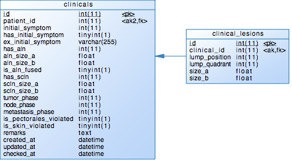
\includegraphics{figure/chap3-5_clinicals.png}
  \bicaption[临床指标]
    {临床指标}
    {schema of clinicals}
  \label{fig:ch3-5}
\end{figure}


\begin{figure}[!htp]
  \centering
  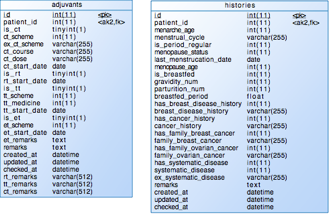
\includegraphics{figure/chap3-4_histories.png}
  \bicaption[辅助治疗和既往病史]
    {辅助治疗和既往病史}
    {schema of  and histories }
  \label{fig:ch3-4}
\end{figure}


\begin{figure}[!htp]
  \centering
  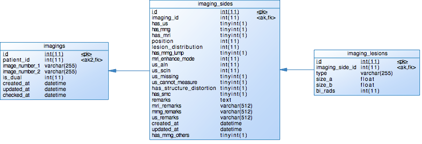
\includegraphics{figure/chap3-3_imagines.png}
  \bicaption[医学影像学检查]
    {医学影像学检查}
    {schema of imagines}
  \label{fig:ch3-3}
\end{figure}


\begin{figure}[!htp]
  \centering
  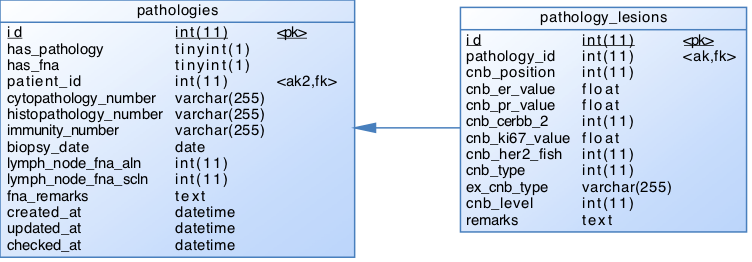
\includegraphics{figure/chap3-2_pathologies.png}
  \bicaption[组织活检病理学]
    {组织活检病理学}
    {schema of pathologies}
  \label{fig:ch3-2}
\end{figure}

\begin{table}[!hpb]
  \centering
  \bicaption[各表结构图索引]
    {各表结构图索引}
    {index of structure of each schema}
  \label{tab:3-1}
  \begin{tabular}{@{}llr@{}} \toprule

    表名 & 与患者表的关系 & 索引\\ \midrule
    % 新辅助治疗方案 & 1 to 1 & 图\ref{fig:ch3-7} \\
    手术病理 & 1 to 1 & 图\ref{fig:ch3-6} \\
    手术病灶 & multi to 1 & 图\ref{fig:ch3-6} \\
    随访记录 & multi to 1 & 图\ref{fig:ch3-6} \\
    临床指标 & 1 to 1 & 图\ref{fig:ch3-5} \\
    既往病史 & 1 to 1 & 图\ref{fig:ch3-4} \\
    辅助治疗方案 & 1 to 1 & 图\ref{fig:ch3-4} \\
    医学影像学检查 & 1 to 1 & 图\ref{fig:ch3-3} \\
    组织活检病理学 & 1 to 1 & 图\ref{fig:ch3-2} \\ \bottomrule
  \end{tabular}
\end{table}

\subsection{病例信息的分类}
\label{para:chap3-1-3}
本文在上一小节详细的介绍了病例数据库的结构,各个表的表项以及其相应的数据类型。在整个数据库中,每个患者都有唯一一个ID,而在每个表中都有相应的记录与之相关联。每一个患者的所有相关信息可以分为两大类:\textbf{患者属性}与\textbf{治疗方案}。

\begin{itemize}

\item \textbf{患者属性}

患者属性是可以用来帮助医生决定其治疗方案的所有表项构成的集合。所有这些属性来源于基本信息表,新辅助治疗表,手术病理表,手术病灶表,临床指标表,既往病史表,医学影像学检查表以及组织病理学表。上述各表的共有特征在于,这些表里面的信息都表达的是病人本身的特性,都来源于科学的检查方法,与客观因素无关。医生对患者的状况的判断,对患者疾病的诊断,甚至于对患者治疗方案的选择全部依赖于这些表中的有关信息。

\item \textbf{治疗方案}

治疗方案是医生针对每一个患者的每一种治疗类型选择的最佳治疗方案。具体的治疗类型有以下四种:

\begin{itemize}

\item 化学治疗,Chemotherapy,记为CT
\item 放射治疗,Radiotherapy,记为RT
\item 靶向治疗,Targeted therapy,记为TT
\item 内分泌治疗,Endocrine therapy,记为ET

\end{itemize}

对于每一种治疗类型,都有一个事先定义好的治疗方案集合。每个集合中的每个治疗方案都定义了该治疗方案的疗程数和用药情况。这些治疗方案都源于医学界多年的经验积累,结合了大量的理论研究与临床试验,已经变得相当成熟。医生仅仅根据患者的属性,为其选择最合适的治疗方案,并不会改变相应类型的治疗方案的详细计划。根据这个特点,可以把患者医疗方案的推荐视为一个多分类问题。这极大地简化了本文后续提到的推荐模型。

\end{itemize}

\section{基于规则的推荐方法}

\subsection{规则来源}
基于规则的推荐方法本质上采用了决策树算法。为患者决策最优化学治疗方案;或者放射治疗方案;或者靶向治疗方案;或者内分泌治疗方案,都可以理解为在决策树中不断选取最优的孩子结点,直到最后到达叶子结点的过程。决策树中的每个叶子结点都对应一种治疗方案。本文中所使用到的规则均来源于规范的医疗指南而没有使用决策树构建算法从数据库中学习。所使用的规则分别来源于NCCN与RJ Guidelines。

NCCN(The National Comprehensive Cancer Network,国家综合癌症网络)是由28个致力于患者护理,研究和教育的领先癌症中心组成的非营利联盟。NCCN致力于改善和促进癌症治疗的质量,提供高效的癌症护理手段,从改善患者的生存质量。  通过定义和推进高质量的癌症护理,NCCN促进了持续质量的改进,并认识到创建适用于全球患者,临床医生和其他医疗保健决策者的临床实践指南的重要性。因此通过NCCN成员机构临床专家的领导和专业知识,NCCN开发了可向卫生保健提供系统中众多利益相关方提供有价值的信息资源。这些信息资源便是NCCN癌症临床实践指南(NCCN Guidelines)\cite{Lyman2005Guidelines}。该指南在医学界被认为是癌症临床治疗的标准。NCCN指南在整个医学界无疑是最权威的且更新速度最快的指南。

而针对乳腺癌这一种癌症,上海交通大学附属瑞金医院乳腺中心提出了一套完备的治疗指南(RJ Guidelines,瑞金指南)。作为国内乳腺疾病领域最为权威的治疗中心,瑞金指南具有重要的参考价值。另外还有一些知名医疗机构也出台了相应的指南,比如ESMO(European Society for Medical Oncology)。

\subsection{基于规则的推荐算法}
本文使用到的基于规则的推荐方法综合了NCCN有关乳腺癌治疗部分的规则以及瑞金乳腺中心制定的规则。这两种规则分别对应了两套规则体系。每个规则体系下的每一个规则都可以视为一个决策树。比如,图\ref{fig:ch3-4}是NCCN乳腺癌治疗指南中的某一条规则,该图片截取自NCCN官方网站\footnote{\url{https://www.nccn.org/}}。此时,假设某个患者具有如下的一系列属性:
\begin{center}
Histology=Mixed term=pT1 tumor\_size=0.7cm
\end{center}
则该患者根据决策树的路径匹配原则刚好可以找到一条由该决策树的根结点到叶子结点的通路。因此该患者的基于规则的推荐结果是"consider adjuvant chemotherapy"。这个决策结果以及做出该决策所依据的相关规则便可以直观的展示给医生。

在\ref{sec_3_1}节介绍过,有数十个属性用来描述一个患者。而上面这个例子中,病人的其他属性并没有被展示,这说明规则的匹配往往只依赖与几个属性。同时,某个患者针对某种治疗类型,在某个规则体系(比如NCCN规则体系,瑞金规则体系)下只有可能有一条规则与之匹配。如果某个患者在某个规则体系下匹配了两条或两条以上的规则,则表明在该规则体系下,这两条规则是相互矛盾的。

\begin{figure}[!htp]
  \centering
  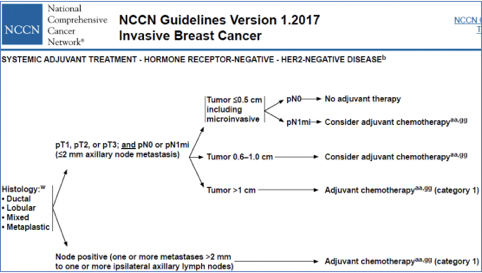
\includegraphics[height=6cm,width=10cm]{figure/chap3-8.png}
  \bicaption[一条NCCN乳腺癌规则]
    {一条NCCN乳腺癌规则}
    {a fragment of NCCN guideline on breast cancer}
  \label{fig:ch3-4}
\end{figure}

对某个患者使用基于规则的推荐方法决策其某种治疗某个治疗类型的治疗方案,具体的过程如算法\ref{algo:3-1}所示。在此算法中,病人的属性在输入后,分别与NCCN和瑞金两大规则体系进行比对,然后输出决策结果。这里存在的问题是,算法针对某种治疗类型的输出可能为空。考虑某个患者有60个属性均为有效值,并假设这些属性都为离散类型并且只有n种可能的取值。假设患者完全由这个属性集描述,则共有$n^{60}$种不同的组合。这个数字与有限的规则数量形成了巨大的反差。表\ref{tab:3-2}



\begin{table}[!hpb]
  \centering
  \bicaption[规则统计信息]
    {规则统计信息}
    {The statical imformation of rules}
  \label{tab:3-2}
  \begin{tabular}{@{}lllllr@{}} \toprule

      & CT & RT & TT & ET & 总数\\ 

    NCCN & 29 & 6 & 9 & 6 & 50 \\
    RJ & 18 & 12 & 8 & 12 & 50 \\ \midrule
    总数 & 47 & 18 & 17 & 18 & 100 \\

  \end{tabular}
\end{table}




\begin{algorithm}
% \begin{algorithm}[H] % 强制定位
\caption{基于规则的治疗方案推荐算法}
\label{algo:3-1}
\begin{algorithmic}[1] %每行显示行号
\Require 某个患者及其所有属性集合X,治疗类型t,其中${t \in \{CT,ET,RT,TT\}}$,NCCN中与t有关的规则集${NCCN_t}$,瑞金指南中与t有关的规则集${RJ_t}$
\Ensure 针对该治疗类型,两种规则体系下的决策结果${RES_{NCCN}}$,${RES_{RJ}}$

\For{X in ${NCCN_t}$}
    \If {X 在该规则中有可以到达的叶子结点}
        \State $ RES_{NCCN} \gets \text{叶子结点对应的决策结果} $
        \State $ break $
    \EndIf
\EndFor

\For{X in ${RJ_t}$}
    \If {X 在该规则中有可以到达的叶子结点}
        \State $ RES_{RJ} \gets \text{叶子结点对应的决策结果} $
        \State $ break $
    \EndIf
\EndFor


\end{algorithmic}
\end{algorithm}


